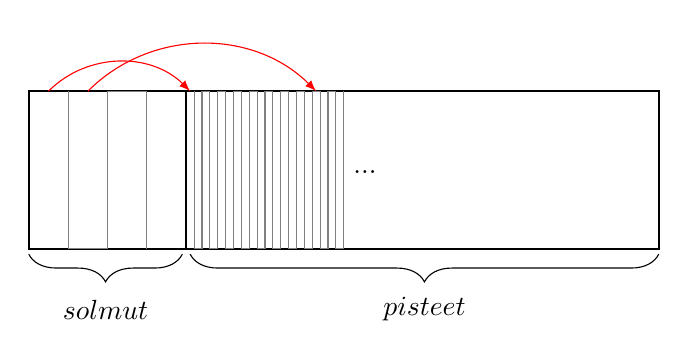
\begin{tikzpicture}
    \draw[thick](0,2,2)--(8,2,2)--(8,0,2)--(0,0,2)--(0,2,2)--(2,2,2)--(2,0,2);
    \draw[gray](0.5,2,2)--(0.5,0,2)--(1,0,2)--(1,2,2)--(1.5,2,2)--(1.5,0,2);
    \draw[gray](2.1,2,2)--(2.1,0,2)--(2.2,0,2)--(2.2,2,2)--(2.3,2,2)--(2.3,0,2)--(2.4,0,2)--(2.4,2,2)--(2.5,2,2)--(2.5,0,2)--(2.6,0,2)--(2.6,2,2)--(2.7,2,2)--(2.7,0,2)--(2.8,0,2)--(2.8,2,2)--(2.9,2,2)--(2.9,0,2)--(3.0,0,2)--(3.0,2,2)--(3.1,2,2)--(3.1,0,2)--(3.2,0,2)--(3.2,2,2)--(3.3,2,2)--(3.3,0,2)--(3.4,0,2)--(3.4,2,2)--(3.5,2,2)--(3.5,0,2)--(3.6,0,2)--(3.6,2,2)--(3.7,2,2)--(3.7,0,2)--(3.8,0,2)--(3.8,2,2)--(3.9,2,2)--(3.9,0,2)--(4.0,0,2)--(4.0,2,2);
    
    \draw[red, -latex](0.25,2,2) to [bend left=45] (2.05,2,2);
    \draw[red, -latex](0.75,2,2) to [bend left=45] (3.65,2,2);
    %\draw[red, -latex](1.25,2,2) to [bend left=45] (5.65,2,2);
    %\draw[red, -latex](1.75,2,2) to [bend left=35] (7.65,2,2);
  
  \node at (3.5,0.2,0) {...};
  
  \draw [decorate,decoration={brace,amplitude=10pt, mirror},xshift=0pt,yshift=-2pt]
  (0,0,2) -- (1.95,0,2)node [black,midway,yshift=-20pt] {$solmut$};
  \draw [decorate,decoration={brace,amplitude=10pt, mirror},xshift=0pt,yshift=-2pt]
  (2.05,0,2) -- (8,0,2)node [black,midway,yshift=-20pt] {$pisteet$};
    
\end{tikzpicture}